\subsubsection{Sequence Diagram - Module Công tác Xã hội}

    Để minh họa chi tiết tương tác giữa các thành phần trong hệ thống, báo cáo trình bày 2 Sequence Diagram đại diện cho các luồng xử lý quan trọng trong module Công tác Xã hội:
    
    \begin{itemize}
        \item \textbf{Tạo và chỉnh sửa hoạt động:} Tương tác giữa người dùng, controller, service layer và database khi tạo/cập nhật hoạt động với logic quản lý trạng thái
        \item \textbf{Chấm điểm từ Excel:} Tương tác phức tạp giữa nhiều component trong quá trình xử lý file Excel hàng loạt, bao gồm file parsing, validation và batch update
    \end{itemize}

    Mỗi diagram thể hiện chi tiết các message trao đổi giữa các đối tượng, thứ tự thực hiện các phương thức, và cơ chế xử lý dữ liệu trong từng bước.

    % ========================================
    % Sequence Diagram - Tạo và chỉnh sửa hoạt động
    \newpage
    \begin{figure}[H]
        \centering
        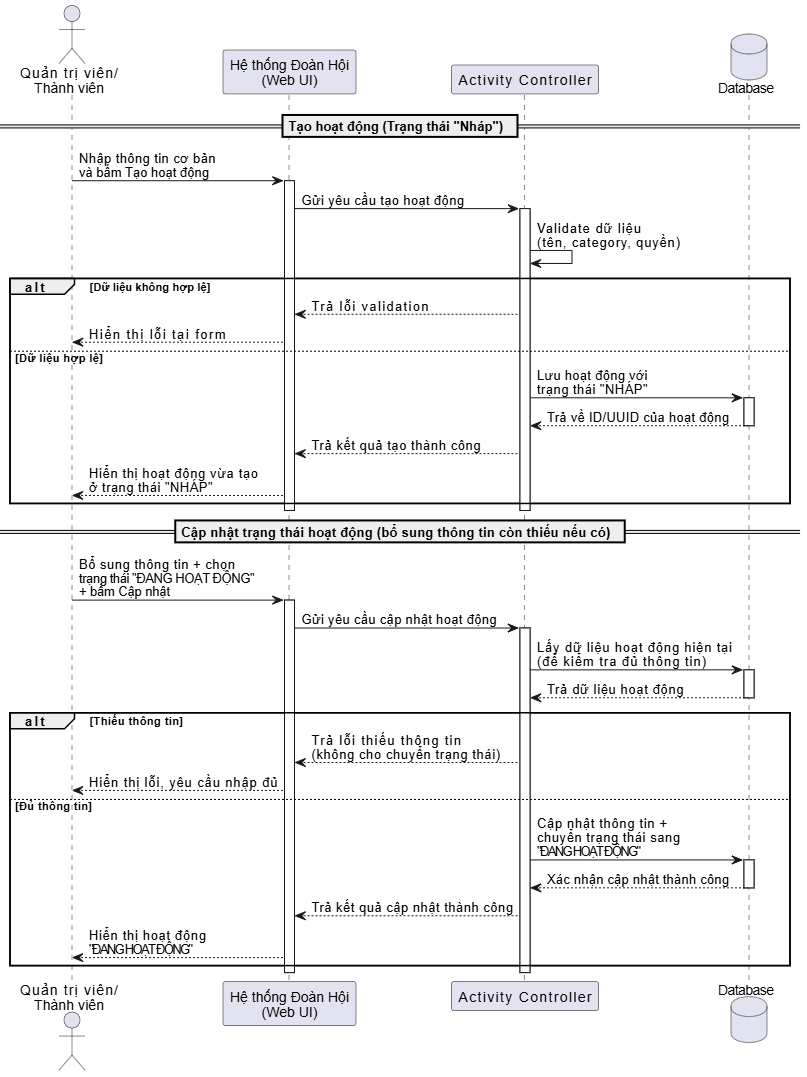
\includegraphics[width=0.95\linewidth]{Images/sequence-diagram/UC07_03_tao_chinh_sua_hoat_dong.png}
        \vspace{0.3em}
        \captionsetup{skip=8pt}
        \caption{Sequence Diagram - Tạo và chỉnh sửa hoạt động CTXH}
        \label{fig:sequence-uc07-03}
    \end{figure}

    Sequence Diagram trên mô tả tương tác giữa các thành phần khi tạo hoặc chỉnh sửa hoạt động CTXH. Actor (Quản trị viên/Người dùng) gửi request qua Controller, Controller gọi Service Layer để xử lý business logic. Service kiểm tra quyền, validate dữ liệu đầu vào (tên không trống, thời gian hợp lệ, số ngày là bội 0.5), và kiểm tra cấu hình giới hạn từ ConfigService. Nếu trạng thái là "Đang hoạt động", Service validate đầy đủ thông tin bắt buộc. Sau khi validation thành công, Service gọi Repository để lưu vào database và trả về kết quả cho người dùng. Nếu có lỗi validation, hệ thống trả về error message cụ thể để người dùng sửa lại.

    % ========================================
    % Sequence Diagram - Chấm điểm từ Excel
    \newpage
    \begin{figure}[H]
        \centering
        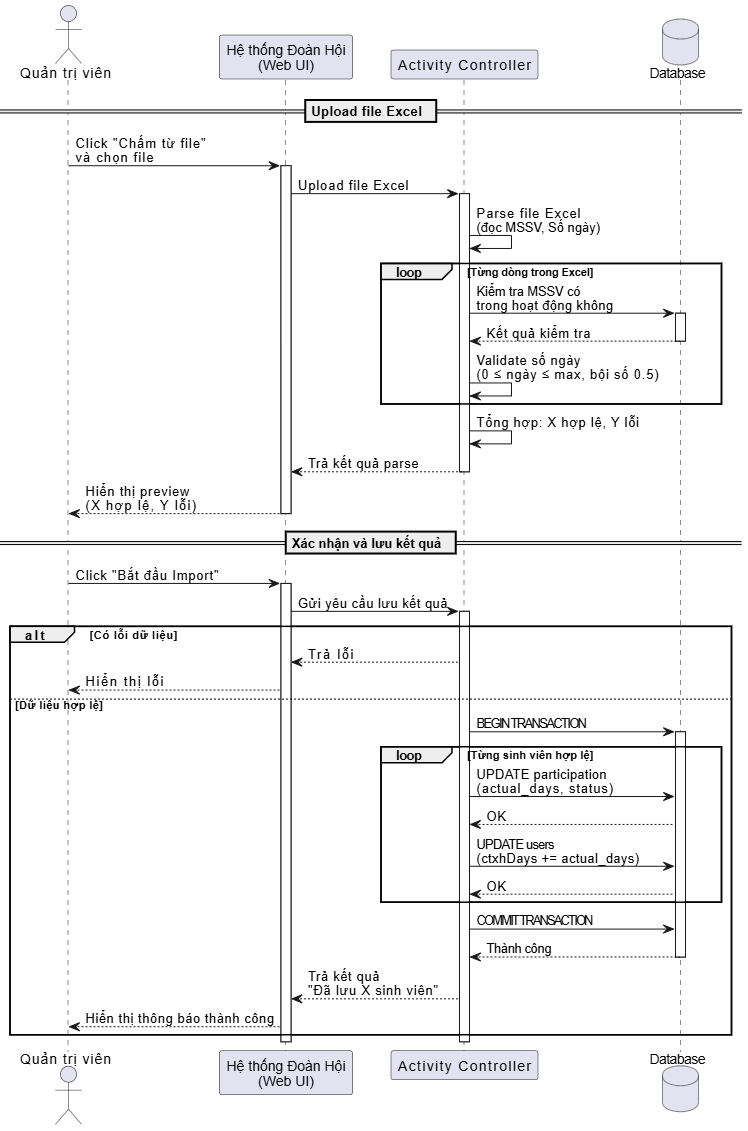
\includegraphics[width=0.95\linewidth]{Images/sequence-diagram/UC07_02_cham_diem_excel.png}
        \vspace{0.3em}
        \captionsetup{skip=8pt}
        \caption{Sequence Diagram - Chấm điểm sinh viên từ file Excel}
        \label{fig:sequence-uc07-02}
    \end{figure}

    Sequence Diagram thể hiện luồng xử lý phức tạp khi chấm điểm hàng loạt từ Excel. Controller nhận file upload, gọi ExcelParserService để parse file thành chunks (500 rows/chunk). Với mỗi chunk, ValidationService validate từng row: kiểm tra sinh viên tồn tại trong database, số ngày hợp lệ (bội 0.5, không âm), và không vượt giới hạn hoạt động. Kết quả validation được trả về dạng preview (danh sách row hợp lệ và row lỗi với lý do). Khi người dùng xác nhận, Service bắt đầu batch update trong transaction: với mỗi row hợp lệ, cập nhật điểm tham gia và cộng vào tổng CTXH của sinh viên. Nếu có lỗi trong quá trình update, toàn bộ transaction được rollback để đảm bảo tính nhất quán dữ liệu. Kết quả cuối cùng (số lượng sinh viên đã cập nhật) được trả về cho người dùng.
